\documentclass[11pt]{article}
\title{\textbf{Meccano pentagons diagonals}}
\author{https://github.com/heptagons/meccano/penta}
\date{}

\usepackage{../meccano}

\begin{document}

\maketitle
\begin{abstract}
We construct meccano\meccanoref regular pentagons internal diagonals.
\end{abstract}

\section{Regular pentagon diagonals}

\begin{figure}[H]
\centering
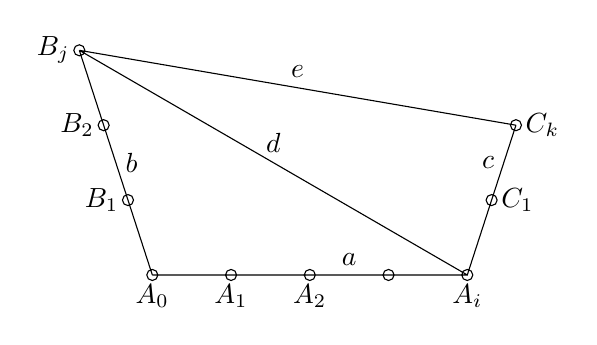
\begin{tikzpicture}
\begin{scope}[scale=1]
\begin{scope}
\draw[] (0,0) circle(2pt) node[below]{$A_i$}
-- ++(-1,0) circle(2pt)
-- node[above]{$a$} ++(-1,0) circle(2pt) node[below]{$A_2$}
-- ++(-1,0) circle(2pt) node[below]{$A_1$}
-- ++(-1,0) circle(2pt) node[below]{$A_0$}
-- ++(108:1) circle(2pt) node[left]{$B_1$}
-- node[right]{$b$} ++(108:1) circle(2pt) node[left]{$B_2$}
-- ++(108:1) circle(2pt) node[left]{$B_j$}
-- node[above]{$d$} (0,0)
-- ++(72:1) circle(2pt) node[right]{$C_1$}
-- node[left]{$c$} ++(72:1) circle(2pt) node[right]{$C_k$}
-- node[above]{$e$} ++(-5.545,0.951); % (-4-5*cos(72M),sin(72))
\end{scope}
\end{scope}
\end{tikzpicture}
\caption{Regular pentagon basic diagonals $d$ and $e$ from sides segments $a\ge\ b\ge c$.}
\label{fig:diagonals}
\end{figure}

From figure \ref{fig:diagonals} we know the regular internal pentagons angle is $\theta = 3\pi/5$:
\begin{align}
\alpha &= \angle{A_0A_iB_j} \\
\beta  &= \angle{B_jA_iC_k} \\
\theta &= \angle{B_jA_0A_i} \\
  &= \alpha + \beta \\
\cos\theta &= \frac{1-\sqrt{5}}{4}\\
\sin\theta &= \frac{\sqrt{10+2\sqrt{5}}}{4}
\end{align}

We use the cosines sum identity to express $\cos\beta$ in function of the rest of variables:
\begin{align}
\cos(\alpha + \beta) &= \cos\theta\\
 &= \cos\alpha\cos\beta - \sin\alpha\sin\beta\\
\sin\beta &= \frac{\cos\alpha\cos\beta - \cos\theta}{\sin\alpha}\\
\sin^2\beta &= \frac{(\cos\alpha\cos\beta - \cos\theta)^2}{\sin^2\alpha}\\
1 - \cos^2\beta &= \frac{\cos^2\alpha\cos^2\beta - 2\cos\alpha\cos\beta\cos\theta + \cos^2\theta}{sin^2\alpha}
\end{align}
We set $X = \cos\beta$ and rearrange the last equation to get:
\begin{align}
\sin^2\alpha X^2 - 2\cos\alpha\cos\theta X + \cos^2\alpha\cos^2\beta + cos^2\theta - \sin^2\alpha &= 0
\end{align}
And solve the quadratic equation $AX^2 + BX + C = 0$ to get $\cos\beta$:
\begin{align}
\cos\beta &= \frac{-B \pm \sqrt{B^2 - 4AC}}{2A}\nonumber\\
 &= \frac{2\cos\alpha\cos\theta \pm 
 \sqrt{(2\cos\alpha\cos\theta)^2 - 4\sin^2\alpha(\cos^2\alpha\cos^2\beta + cos^2\theta - \sin^2\alpha)}}
 {2\sin^2\alpha}\nonumber\\
 &= \frac{\cos\alpha\cos\theta \pm 
 \sqrt{\cos^2\alpha\cos^2\theta - \sin^2\alpha(\cos^2\alpha\cos^2\beta + cos^2\theta - \sin^2\alpha)}}
 {\sin^2\alpha}\nonumber\\
\end{align}













From the law of cosines we calculate distance $d$ from integers $a,b$ which equal respectively to
iterators $i,j$:
\begin{align}
d &= \sqrt{a^2 + b^2 - 2ab\cos\theta} \nonumber\\
 &= \sqrt{a^2 + b^2 - 2ab\left(\frac{1-\sqrt{5}}{4}\right)} \nonumber\\
 &= \frac{\sqrt{4a^2 + 4b^2 - 2ab +2ab\sqrt{5}}}{2}
\end{align}











Using the law of cosines we calculate the angles $\alpha =\angle{A_0A_iB_j}$ 
and $\beta =\angle{B_jA_iC_k}$:
\begin{align}
\cos\alpha &= \frac{a^2 + d^2 - b^2}{2ad} \\
 &= \frac{a^2 + (a^2 + b^2 - 2ab\cos\theta) - b^2}{2ad}\nonumber \\
 &= \frac{a - b\cos\theta}{d}\\
%
\cos\beta &= \frac{c^2 + d^2 - e^2}{2cd}\nonumber\\
 &= \frac{c^2 + (a^2 + b^2 - 2ab\cos\theta) - e^2}{2cd}\nonumber\\
 &= \frac{a^2 + b^2 + c^2 - e^2 - 2ab\cos\theta}{2cd}
\end{align}
We define new variable $f$ to simplify $\cos\beta$ to obtain:
\begin{align}
f &\equiv \frac{a^2 + b^2 + c^2 - e^2}{2} \\
\cos\beta &= \frac{f - ab\cos\theta}{cd}
\end{align}

We calculate $\sin\alpha = \sqrt{1 - \cos^2\alpha}$:
\begin{align}
\sin\alpha &= \sqrt{1 - \frac{(a - b\cos\theta)^2}{d^2}}\nonumber\\
 &=\frac{\sqrt{d^2 - a^2 + 2ab\cos\theta - b^2\cos\theta^2}}{d}\nonumber\\
 &=\frac{\sqrt{(a^2 + b^2 - 2ab\cos\theta) - a^2 + 2ab\cos\theta - b^2\cos^2\theta}}{d}\nonumber\\
 &=\frac{\sqrt{b^2(1-\cos^2\theta)}}{d}\nonumber\\
 &=\frac{b\sin\theta}{d}\\
\end{align}



%We define two integers $m, n$ to simplify last equation and obtain:
%\begin{align}
%m &= 4a^2 + 4b^2 - 2ab \\
%n &= 2ab \\
%d &= \frac{\sqrt{m + n\sqrt{5}}}{2}
%\end{align}


%We substitute the cosine and denominator with the surds values and move any surd to numerator:
%\begin{align}
%\cos\alpha &= \frac{a - b\left(\frac{1-\sqrt{5}}{4}\right)}{\frac{1}{2}\sqrt{m + n\sqrt{5}}} \\
% &= \frac{(4a - b + b\sqrt{5})\sqrt{m + n\sqrt{5}}}{2(m + n\sqrt{5})} \nonumber\\
% &= \frac{(4a - b + b\sqrt{5})(m - n\sqrt{5})\sqrt{m + n\sqrt{5}}}{2(m^2 - 5n^2)} \nonumber\\
% &= \frac{\left(4am -bm - 5bn +(bn + bm -4an)\sqrt{5}\right)\sqrt{m + n\sqrt{5}}}{2(m^2 - 5n^2)}
%\end{align}
%We define new integers $p,q,r$ to simplify $\cos\alpha$:
%\begin{align}
%4p &= 4am - bm - 5bn\nonumber\\
% &= 4a(4a^2 + 4b^2 - 2ab) - b(4a^2 + 4b^2 - 2ab) - 5b(2ab)\nonumber\\
% &= 16a^3 + 16ab^2 - 8a^2b - 4a^2b - 4b^3 + 2ab^2 - 10ab^2\nonumber\\
% &= 4(4a^3 - 3a^2b + 2ab^2 - b^3)\nonumber\\
%p &= 4a^3 - 3a^2b + 2ab^2 - b^3\\
%%
%4q &= bn + bm - 4an\nonumber\\
% &= b(2ab) + b(4a^2 + 4b^2 - 2ab) - 4a(2ab)\nonumber\\
% &= 2ab^2 + 4a^2b + 4b^3 - 2ab^2 - 8a^2b\nonumber\\
% &= -4b(a^2 - b^2)\nonumber\\
%q &= -4(a^2 - b^2)\\
%%
%16r &= m^2 - 5n^2\nonumber\\
% &= (4a^2 + 4b^2 - 2ab)^2 - 5(2ab)^2\nonumber\\
% &= 16(a^4 - a^3b + a^2b^2 - ab^3 + b^4)\nonumber\\
%r &= a^4 - a^3b + a^2b^2 - ab^3 + b^4\\
%\end{align}
%We substitute $p,q,r$:
%\begin{align}
%\cos\alpha &= \frac{4\left(p+q\sqrt{5}\right)\sqrt{m + n\sqrt{5}}}{32r}\nonumber\\
% &= \frac{\sqrt{(p+q\sqrt{5})^2(m + n\sqrt{5})}}{8r}\nonumber\\
% &= \frac{\sqrt{mp^2 + 5mq^2 + 10npq + (2mpq + np^2 + 5nq^2)\sqrt{5}}}{8r}
%\end{align}


\end{document}
